
\documentclass[tikz]{standalone}
\usepackage{pgfplots}
\usepackage{tikz}
\usetikzlibrary{arrows}
\usetikzlibrary{backgrounds}
\usetikzlibrary{positioning,calc,quotes}
\usetikzlibrary{shapes.arrows, arrows.meta}

\begin{document}

% \begin{figure}[!h]
% \centering
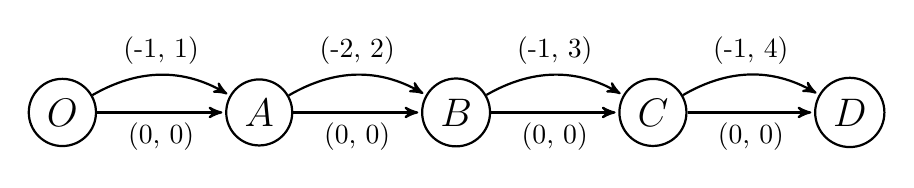
\begin{tikzpicture}[->,>=stealth',shorten >=1pt,auto,node distance=2.5cm,
% \begin{tikzpicture}[-,shorten >=1pt,auto,node distance=3cm,
thick,main node/.style={circle,draw,font=\sffamily\Large\bfseries}]

\node[main node] (O) {$O$};
\node[main node] (A) [right of=O] {$A$} ;
% \node[main node] (B) [below right of=O] {$C$} ;
\node[main node] (B) [right of=A] {$B$};
\node[main node] (C) [right of=B] {$C$} ;
\node[main node] (D) [right of=C] {$D$} ;
% \node[main node] (E) [below right of=B] {$E$} ;
    



\path[]
(O) edge [bend left]  node [above, rotate=0] {(-1, 1)}  (A) 
(O) edge []  node [below, rotate=0] {(0, 0)}  (A) 
(A) edge [bend left] node [above, rotate=0] {(-2, 2)}  (B) 
(A) edge  node [below, rotate=0] {(0, 0)}  (B) 

(B) edge [bend left] node [above, rotate=0] {(-1, 3)}  (C) 
(B) edge  node [below, rotate=0] {(0, 0)}  (C) 

(C) edge [bend left] node [above, rotate=0] {(-1, 4)}  (D) 
(C) edge  node [below, rotate=0] {(0, 0)}  (D) 
% (O) edge  node [below, rotate=0] {4}  (C) 
% (O) edge  node [below, rotate=0] {10}  (D) 
% (A) edge  node [below, rotate=0] {2}  (C) 
% (C) edge  node [right, rotate=0] {-1}  (D) 
% (B) edge  node [below, rotate=0] {5}  (D) 
;
            
\end{tikzpicture}
    % \caption{The network for Problem 2.}
    % \label{fig:enter-label}
% \end{figure}

\end{document}